\chapter{Algorithm Selection \& Autotuning}
\label{chap:autonomous}
\epigraph{\textit{There is nothing like looking, if you want to find something. You
certainly usually find something, if you look, but it is not always quite the
something you were after.}}{--- J.R.R. Tolkien, \textit{The Hobbit}}

This chapter presents the fundamentals and the literature background for the
work described in the case studies of chapter~\ref{chap:usecases}.
Section~\ref{sec:algselres} describes the algorithm selection problem and
the general architecture of autonomous solvers.
Section~\ref{sec:autotuning} presents a literature review of autotuning works
in different domains and using different strategies.
Section~\ref{sec:opentuner} describes the OpenTuner framework, its software
architecture, and the difficulties we had in applying parallel and distributed
programming models to it.

\section{Algorithm Selection}
\label{sec:algselres}

In 1976 John R. Rice published \textit{The Algorithm Selection
Problem}~\cite{rice1976algorithm}, an influential paper where he formulated
abstract models for the problem of selecting effective algorithms for a given
problem. The four main components of the abstract model are the \textit{problem
space} $P$, the \textit{feature space} $\Phi$, the \textit{algorithm space}
$A$, and the \textit{performance space} $\Pi$. The algorithm selection problem
can be formally stated~\cite{smith2009cross} as:

\begin{definition}[The Algorithm Selection Problem]
    For a given problem $x \in P$, with features $f(x) = \phi \in \Phi$,
    find the algorithm selection mapping $s(\phi) = \alpha \in A$, such
    that the selected algorithms minimize the performance mapping
    $p(\alpha,x) = \pi \in \Pi$.
\end{definition}

\begin{figure}[htpb]
    \begin{center}
        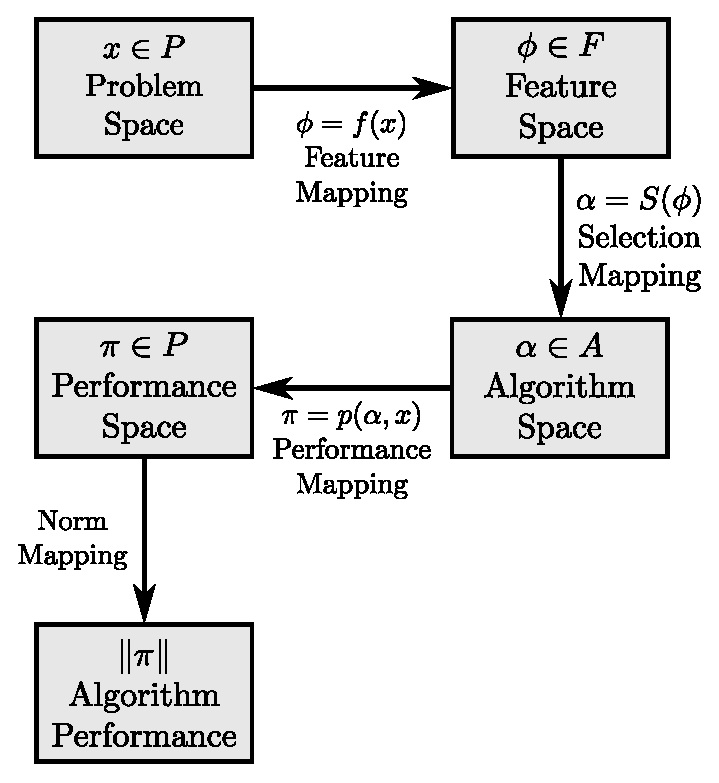
\includegraphics[width=.4\textwidth]{algorithm-selection}
    \end{center}
    \caption{Algorithm Selection Framework, adapted from
    Rice~\cite{rice1976algorithm}}
    \label{fig:riceframe}
\end{figure}

Figure~\ref{fig:riceframe} presents Rice's algorithm selection framework.
Consider a \textit{problem space} $P$, and a problem $x \in P$. The
features of this problem, such as its domain, number of variables and input
size, determine which algorithms are able to solve the problem. The real
problem solving circumstances may also be considered as problem features. For
example, the computer architecture in which the problem will be solved might
define problem features such as limits on accuracy, data accesses, execution
time and memory and power consumption.  The set $\phi$ of features of problem
$x$ is obtained by a feature mapping function $f$, such that $f(x) = \phi \in
\Phi$, where $\Phi$ is the \textit{feature space}.

With the set of features of a problem it is possible to determine which
algorithms can solve the problem. For example, while the insertion sort
algorithm is not useful to sort large arrays if time is a constraint, the
binary tree sort algorithm is not useful if memory is a constraint.  The degree
in which the problem input is already sorted can also be considered a
problem feature. Despite the absence of explicit algorithm parameters and
features in the framework, it is still possible to consider differently
configured versions of an algorithm as distinct algorithms in $A$.  The set
$\alpha$ of algorithms that solve problem $x$ is obtained by a selection
mapping function $s$, such that $s(\phi) = \alpha \in A$, where $A$ is the
\textit{algorithm space}.

After the algorithm set $\alpha$ is defined its performance can be obtained by
empirically measuring metrics of interest, or computing them using an
analytical model or a model trained using machine learning. The set $\pi$ of
performance measurements of the set of algorithms $\alpha$ when solving $x$ is
obtained by a performance mapping function $p$, such that $p(\alpha,x) = \pi
\in \Pi$, where $\Pi$ is the \textit{performance space}.

A normalized performance measurement for the set $\pi$ is obtained by a norm
mapping function. This function can combine measurements of metrics in
different scales or optimization levels, such as execution time, memory and
power consumption, and hardware occupancy and size. The set of normalized
values $||\pi||$ is called the \textit{algorithm performance}.

A new set of algorithms $\alpha{}'$ is obtained by a selection mapping function
$s_{a}$, such that $s_{a}(\phi,\alpha,||\pi||) = \alpha{}' \in A$, where $\phi$
is the set of features, $\alpha$ is the previous algorithm set, and $||\pi||$
is the algorithm performance.

This last step makes it clear that solving the algorithm selection problem can
be seen as an iterative and dynamic process, that improves by considering
previous algorithm selections and their performance measurements. One problem
that surfaces from this framework is finding the selection mapping functions
$s$ and $s_{a}$, which can again be seen as a new instance of the algorithm
selection problem. This new problem can be interpreted, for example, as a
function approximation problem, a learning problem, or a search problem.  It
can therefore be solved by many different strategies.  The work we have done so
far treats the problem of finding selection mapping functions as a search
problem. The next section discusses autonomous solvers, dynamically configured
systems that search for selection mapping functions.

\subsection{Autonomous Solvers}

An autonomous solver is a system capable of reconfiguring its components
according to a set of pre-defined rules and subject to external circumstances.
According to the general architecture of autonomous solvers presented by Hamadi
\emph{et al.}~\cite{hamadi2011autonomous, hamadi2012autonomous} and shown in
Figure~\ref{fig:general_solver}, the components of a solver consist of the
algorithms involved in search, such as heuristics and inference mechanisms.
Hamadi \emph{et al.} define the external circumstances a solver is subject to
as the information collected or computed during search.  The control layer of a
solver is responsible for configuring the solver's internal components.

A solver can use multiple simultaneous search techniques, each with its own
search algorithm, performance model or heuristic. Search techniques apply
operators, such as randomization and perturbation, to points in the search
space, obtaining new points to measure. The selection and ordering of operators
is controlled by the configuration parameters of each search technique.

\begin{figure}[htpb]
    \centering
    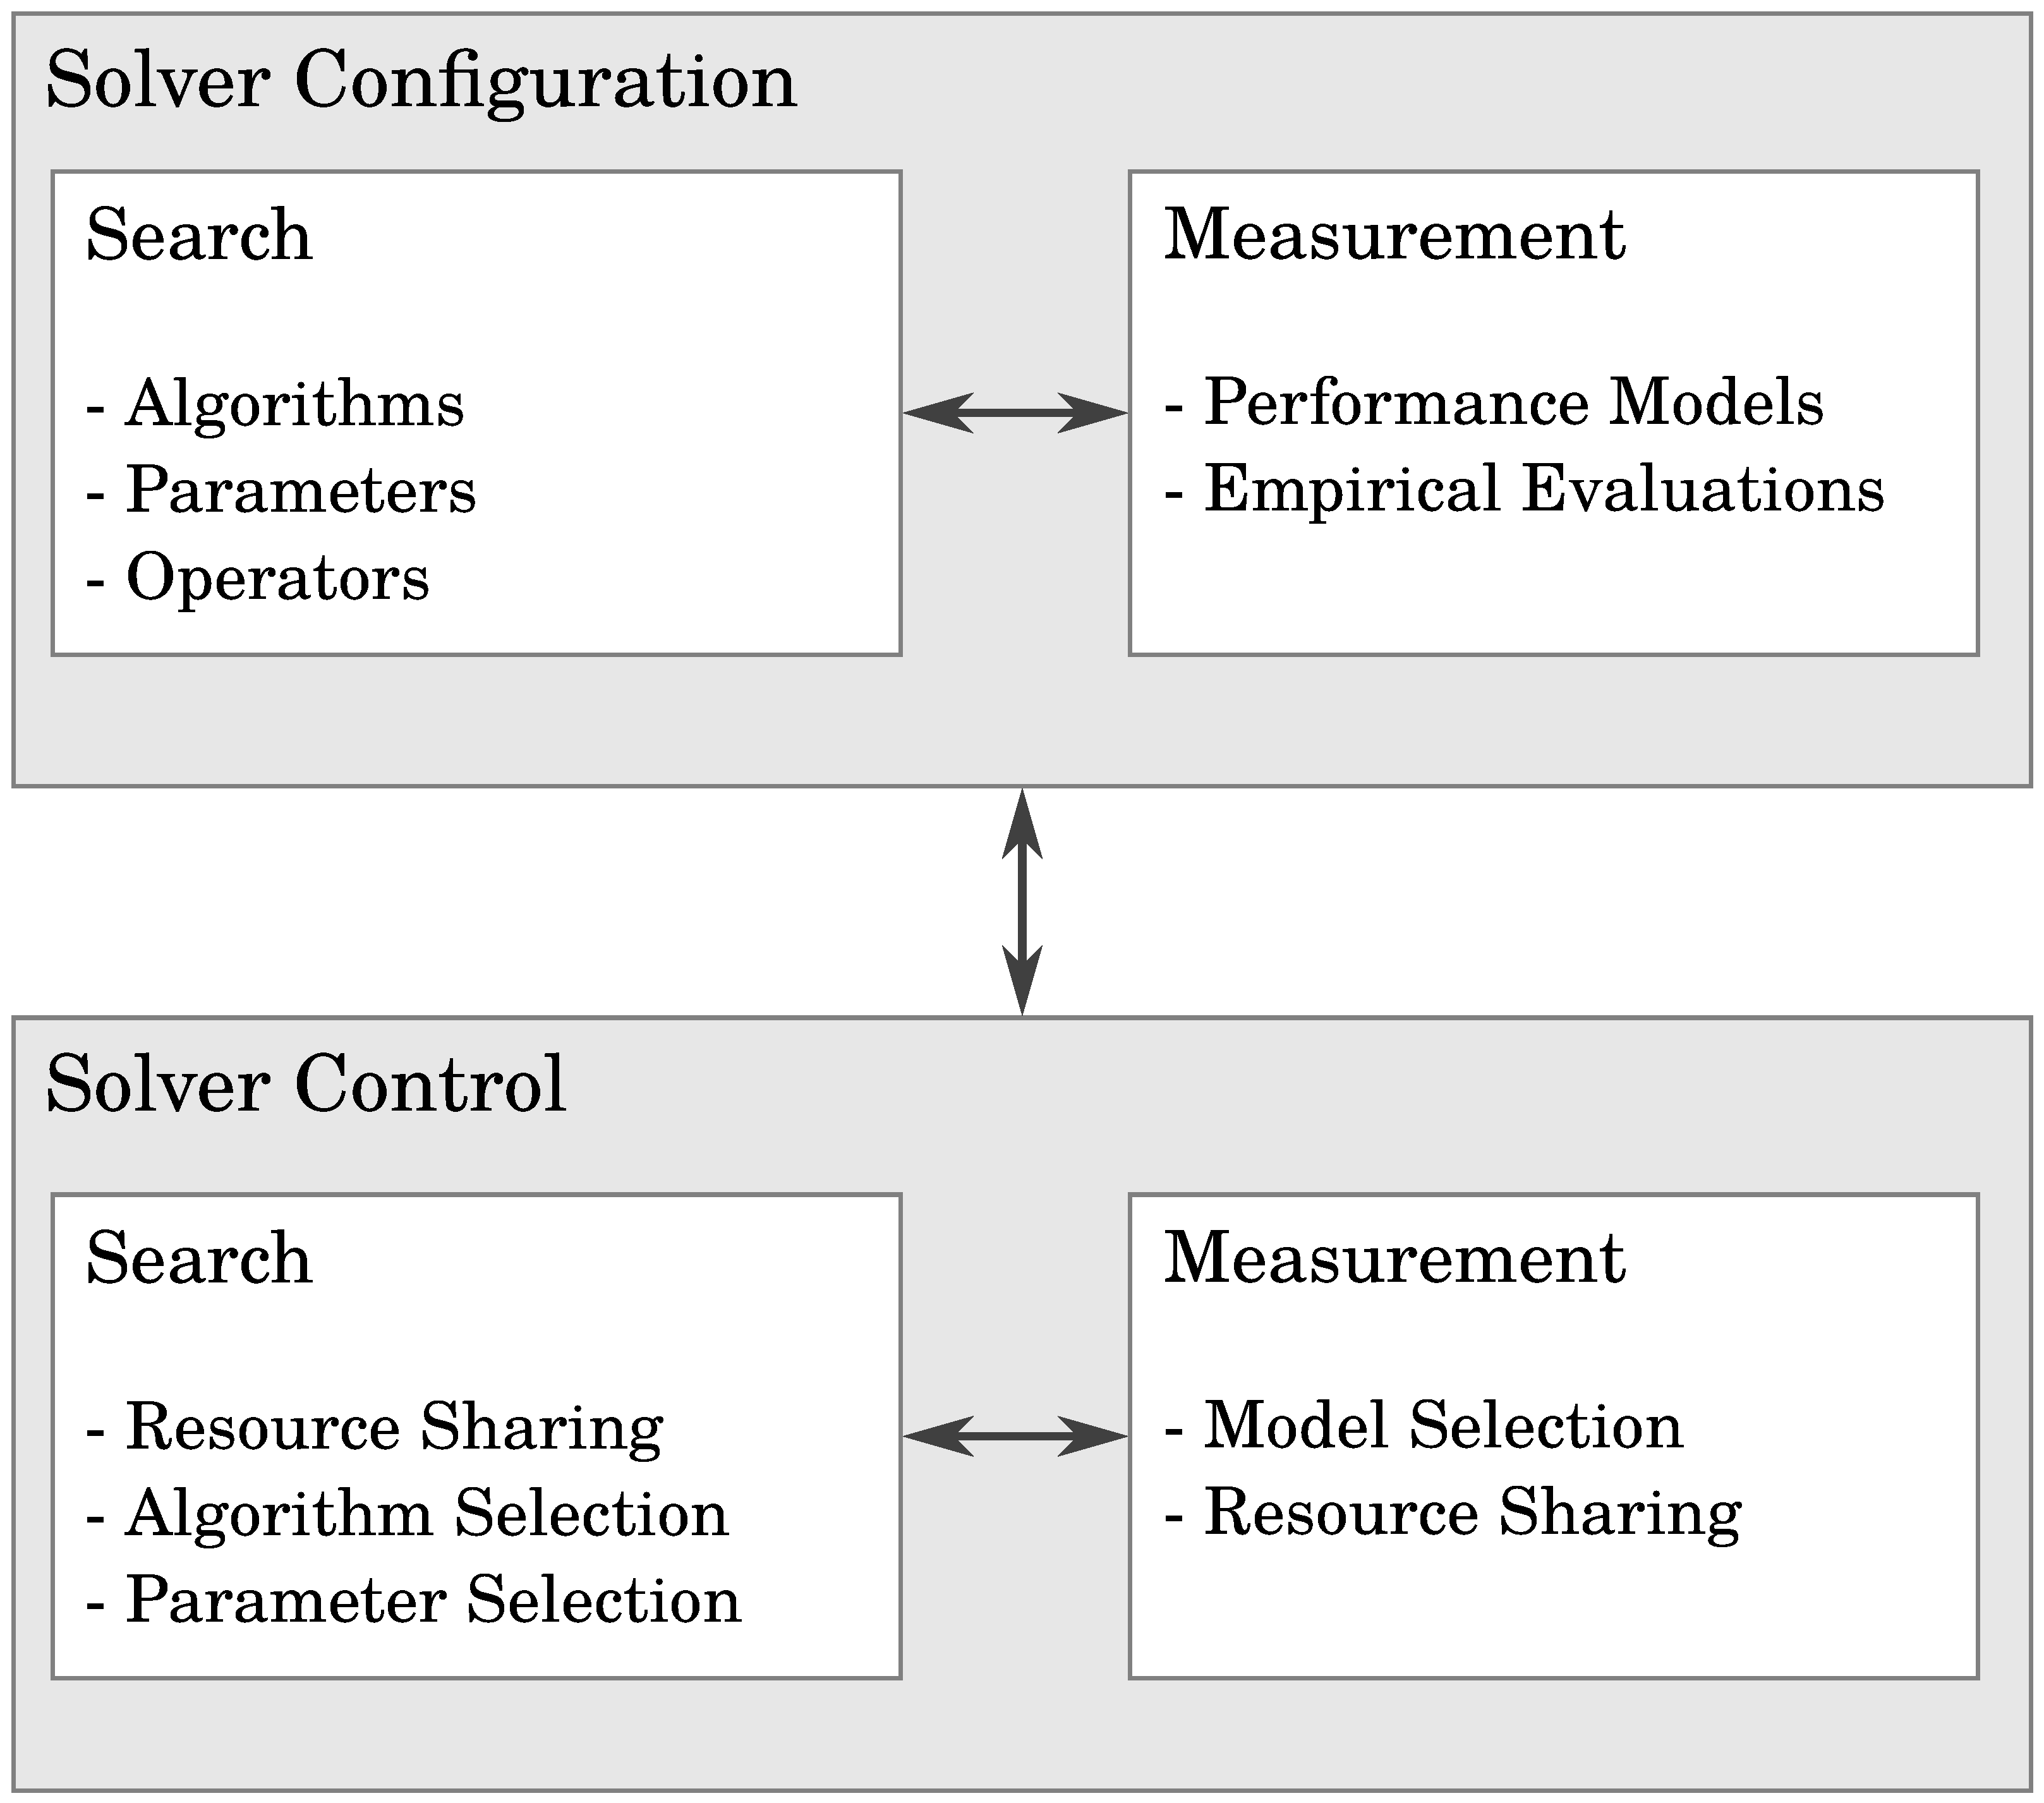
\includegraphics[width=.46\textwidth]{general_solver}
    \caption{General autonomous solver architecture, adapted from Hamadi \emph{et al.}~\cite{hamadi2012autonomous}}
    \label{fig:general_solver}
\end{figure}

Search techniques use performance values associated with points in the
search space to guide their search. These values are measured or computed
using performance or inference models, or empirical evaluations.
Models can be analytically built or trained using machine learning
algorithms, and evaluations are usually done by running the program
with the configuration correspondent to a given point in the search
space, and measuring a software or hardware metric.

The control layer of an autonomous solver is responsible to reconfigure the
search and measurement components, adapting the solver to information
collected during search, such as search space size and local minima, available
computational resources and hardware metrics. The control layer can also use
information computed during search, such as search technique performance over
time and heuristic pruning capacity.

In the search component the control layer can configure search algorithms and
their parameters, select search space dimensions to use in search, and define
operator ordering and computational resource sharing schedules.  In the
measurement component the control layer can select which performance and
inference models will be used for predictions, in which computational resource
the evaluations will be performed, and also resource sharing schedules.

The stage of the target program's execution in which an autonomous solver
operates is a distinctive property. Solvers that search for optimized
parameters of an algorithm by changing parameters during the algorithm's
runtime are called \textit{online} autonomous solvers, and solvers that search
for optimized parameters before runtime, for example, by using test runs with
different parameters, are called \textit{offline} autonomous solvers. In this
work we did not experiment with \textit{online} autonomous solvers, so the
following section does not distinct the two categories, although most of the
work presented there studies \textit{offline} autonomous solvers.

% Final thesis should contain:
%
%\section{On-line Control}
%\label{sec:oncontrol}
%
%\subsection{Adaptive Parameter Configuration}
%\label{subsec:paramadaptive}
%
%\subsection{Credit Assignment}
%\label{subsec:creditassign}
%
%\subsection{Reinforcement Learning}
%\label{subsec:reinforce}
%
%\section{Off-line Configuration}
%\label{sec:offconfig}
%
%\subsection{Evolutionary Computing}
%\label{subsec:evolcomp}
%
%\subsection{Stochastic Local Search}
%\label{subsec:searchsls}
%
%\subsection{Machine Learning}
%\label{subsec:searchml}

\section{Autotuning}
\label{sec:autotuning}

This section presents autotuning systems from different application domains,
categorized by the autotuning strategy they use. We gathered from the Google
Scholar bibliographic database the most relevant autotuning systems published
in the years of 2015, 2016 and 2017. We also briefly discuss notable autotuning
systems published before 2015.

The categories of autotuning strategies we use in this section are
\textit{Search Algorithms \& Heuristics}, \textit{Machine Learning \&
Model-Aided}, and \textit{Combinations}. Figure~\ref{fig:strategies} shows the
relations between the strategies. The intended contribution of this work is a
\textit{Domain-Agnostic System}, and we include this special category at the
end. Since we discuss the OpenTuner framework~\cite{ansel2014opentuner} in more
detail in this chapter, and we also use it in most case studies presented in
chapter~\ref{chap:usecases}, we also list autotuning systems that use it.

\begin{figure}[htpb]
    \centering
    \includegraphics[width=.46\textwidth]{autotuning_strategies}
    \caption{Categories of autotuning strategies discussed in this section}
    \label{fig:strategies}
\end{figure}

Table~\ref{tab:systems} shows a selection of autotuning systems from different
problem domains, using different autotuning techniques. The variety of solutions
and domains makes clear that there is no single solution for all autotuning
problems, strengthening the argument that domain-agnostic autotuning systems
should use a combination of techniques when possible.

Rice's conceptual framework~\cite{rice1976algorithm} forms the foundation for
autotuners in various problem domains.  In 1997, the PHiPAC
system~\cite{bilmes1997optimizing} used code generators and search scripts to
automatically generate high performance code for matrix multiplication. Since
then, systems tackled different domains with a diversity of strategies. Whaley
\emph{et al.}~\cite{dongarra1998automatically} introduced the ATLAS project,
that optimizes dense matrix multiplication routines. The
OSKI~\cite{vuduc2005oski} library provides automatically tuned kernels for
sparse matrices. The FFTW~\cite{frigo1998fftw} library provides tuned C
subroutines for computing the Discrete Fourier Transform.

\begin{table}[htpb]
    \centering
    \begin{tabular}{@{}lll@{}}
        \toprule
        System & Domain & Technique \\ \midrule
        ATLAS~\cite{dongarra1998automatically} & Dense Linear Algebra & Exhaustive \\
        OSKI~\cite{vuduc2005oski} & Sparse Linear Algebra & Heuristic + Exhaustive \\
        LGen~\cite{spampinato2014basic} & Small-scale Linear Algebra & Exhaustive + Random \\
        INSIEME~\cite{jordan2012multi} & Compiler & Genetic Algorithm \\
        Petabricks~\cite{ansel2009petabricks} & Domain-Agnostic & Genetic Algorithm\\
        TANGRAM~\cite{chang2016efficient} & Heterogeneous Architectures & Breadth-First Search + Pruning \\
        Active Harmony~\cite{tapus2002active} & Runtime & Nelder-Mead \\
        MASE-BDI~\cite{coelho2016mase} & Environmental Land Change & Distributed Active Harmony~\cite{tapus2002active} \\
        ParamILS~\cite{hutter2009paramils} & Domain-Agnostic & Stochastic Local Search \\
        CLTune~\cite{nugteren2015cltune} & OpenCL kernels & Stochastic Local Search\\
        OPAL~\cite{audet2014optimization} & Domain-Agnostic & Direct Search \\
        MILEPOST GCC~\cite{fursin2011milepost} & Compiler & Central DB + Machine Learning \\
        Apollo~\cite{beckingsale2017apollo} & GPU kernels & Decision Trees \\
        OpenTuner~\cite{ansel2014opentuner} & Domain-Agnostic & Ensemble \\
        Periscope~\cite{gerndt2017multi} & HPC Applications & Various \\
        \bottomrule
    \end{tabular}
    \caption{Selected autotuning systems, their domains and techniques}
    \label{tab:systems}
\end{table}

\subsection{Search Algorithms \& Heuristics}

A common and still effective strategy for autotuning is to use search
algorithms, which can be simple such as simulated annealing and random walks,
or more elaborated, such as genetic algorithms and particle swarm optimization.
Search heuristics can also be developed and used effectively if an adequate
knowledge of the problem domain is obtained. When using search algorithms and
heuristics, autotuners must empirically evaluate program configurations to find
an optimized configuration. Most search algorithms and heuristics present few
or none convergence guarantees. Works in this category use search
algorithms and heuristics perform autotuning in different problem domains.

Abdelfattah \emph{et al.}~\cite{abdelfattah2016performance} present an
autotuning strategy using exhaustive evaluation of General Matrix-Matrix
Multiply (GEMM) kernel optimizations for GPUs. They later use this approach to
optimize GPU kernels for large-scale tensor
contractions~\cite{abdelfattah2016high}.  Guerreiro \emph{et
al.}~\cite{guerreiro2015multi} use search space pruning strategies and
exhaustive evaluation to autotune CUDA GPU kernels.
LGen~\cite{spampinato2014basic} is a compiler for small-scale linear algebra
computation that uses mathematical domain-specific languages to optimize loops
and vectorization. LGen uses exhaustive or random search to test different
optimizations.

Active Harmony~\cite{tapus2002active} provides an API that enables online
autotuning of a program using a variation of the Nelder-Mead simplex
algorithm~\cite{nelder1965simplex}.  MASE-BDI~\cite{coelho2016mase} is a
multi-agent system for the simulation of environmental land change that uses
the Active Harmony API~\cite{tapus2002active} and its search algorithms to
autotune  simulator parameters.  Several simulator configurations are executed
in parallel and communicate their results to a tuning manager using MPI.
CLTune~\cite{nugteren2015cltune} is an autotuning framework for OpenCL kernels
that uses search algorithms such as simulated annealing and particle swarm
optimization.  In an effort to provide a common representation of multiple
parallel programming models, the INSIEME compiler
project~\cite{jordan2012multi} implements abstractions for OpenMP, MPI and
OpenCL, and generates optimized parallel code for heterogeneous multi-core
architectures using genetic algorithms.

\subsection{Machine Learning \& Model-Aided}

Machine Learning algorithms have been used to solve an increasingly larger set
of Computer Science problems. The role of these algorithms in autotuners is to
build a performance model using a program's parameters, target architecture and
input.  The trained model can suggest new configurations for auxiliary search
algorithms or directly provide optimized configurations.

Tartara and Reghizzi~\cite{tartara2012parallel} use the MapReduce programming
model to improve the performance of machine learning algorithms in the
PetaBricks compiler. Later they presented a machine learning
algorithm~\cite{tartara2013continuous} that learns compiler heuristics using
data gathered after every compilation.  Mametjanov \emph{et
al.}~\cite{mametjanov2015autotuning} present an autotuning approach that uses
machine learning and selective sampling of the search space to optimize FPGA
hardware design parameters for performance and power.

Hou \emph{et al.}~\cite{hou2017auto} present an autotuning framework that uses
decision trees to optimize the sparse matrix-vector multiply kernel for multi
and many-core processors.  Apollo~\cite{beckingsale2017apollo} is an autotuning
framework for input-dependent kernels that uses a decision tree classifier that
provides optimizations that can be selected during runtime. MILEPOST
GCC~\cite{fursin2011milepost} and Collective Mind~\cite{fursin2015collective}
are notable research efforts in autotuning compiler optimizations.  These
projects build a central database of compiler optimizations and performance
metrics from collective experience and use machine learning algorithms to
improve autotuned suggestions.

Falsch and Elster~\cite{falch2017machine} build performance
models for OpenCL applications in different target architectures using machine
learning.  The learned statistical model is later used to pick promising
configurations for testing.  Balaprakash \emph{et
al.}~\cite{balaprakash2016automomml} introduce a framework that uses machine
learning algorithms to build models for metrics such as performance and energy
consumption, which are used for multi-objective optimization.

Autotuners can also use analytical performance models to suggest optimized
configurations.  Lang~\cite{lang2017data} reviews work on autotuning based on
analytical performance models, arguing that the approach is feasible.  Xu
\emph{et al.}~\cite{xu2016analytical} introduce an autotuning framework for
loop scheduling in GPUs that uses analytical performance models.
TuningGenie~\cite{ivanenko2014method} presents an autotuning framework that
uses code annotations and an analytical model for generating autotuners for
parallel programs.

\subsection{Combinations}

Systems in this category combine autotuning strategies from different
categories to improve found configurations and autotuner runtime.  The idea
behind a combination of autotuning techniques is that one strategy will
compensate the other. For example, the autotuner may detect that a random walk
algorithm got stuck in a local minima of the search space, in which point the
autotuner could start using a hill-climbing algorithm.

Garvey \emph{et al.}~\cite{garvey2015automatic} present a strategy to autotune
OpenCL GPU kernels using machine learning, heuristics for search space
partitioning and exhaustive search.  PolyMage~\cite{mullapudi2015polymage} is a
domain-specific language and compiler for image processing pipelines. It uses
heuristics and performance models to prune the search space, which is then
explored exhaustively.  Ziegler \emph{et
al.}~\cite{ziegler2016synthesis,ziegler2016scalable} present an autotuning
system for hardware synthesis parameters that uses genetic and learning
algorithms to explore the hardware design space for real industrial chip
designs from IBM.  Ngoko \emph{et al.}~\cite{ngoko2016automatic} introduce an
autotuning system for $\NP$-hard problems that uses distributed measurements of
configurations and machine learning algorithms aided by randomization,
clustering and set intersection solvers.  Luo \emph{et al.}~\cite{luo2015fast}
present a framework for stencil computations that uses Optimal-Solution Spaces,
input feature extraction and machine learning.

\subsection{Domain-Agnostic Systems}

In this work the Domain-Agnostic category refers to autotuners that provide
general abstractions for the representation of search spaces from different
problem domains. These abstractions are used to represent program parameters
and configurations and enable the implementation of autotuners for various
problem domains. Domain-Agnostic systems must also employ a robust set of
autotuning techniques in order to achieve good performance in different
domains.

Petabricks~\cite{ansel2009petabricks} is a language and compiler that enables
the expression of program implementation search spaces at language level.
OpenTuner~\cite{ansel2014opentuner} is a domain-agnostic autotuning framework
that provides ensembles of search techniques for user-defined program
configurations.  The ParamILS framework~\cite{hutter2009paramils} applies
stochastic local search methods for algorithm configuration and parameter
tuning.  TANGRAM~\cite{chang2015tangram,chang2016efficient} is a kernel
synthesis framework for different architecture hierarchies.  It uses
composition rules and breadth-first search to prune and explore the design
space.  The Periscope Tuning Framework
(PTF)~\cite{gerndt2005periscope,gerndt2010automatic,gerndt2017multi} is an
online tool for performance analysis and tuning that has a modular architecture
based on plugins.  OPAL~\cite{audet2014optimization} is domain-agnostic system
for parameter optimization that uses direct search and is able to run parallel
and distributed measurements.

\subsubsection{Works using OpenTuner}

Since the publication of the OpenTuner in 2014, work in different domains
validated the framework's efficacy in implementing autotuners. Most case
studies we present in chapter~\ref{chap:usecases} also used OpenTuner.

Takizawa \emph{et al.}~\cite{takizawa2017customizable} use
OpenTuner~\cite{ansel2014opentuner} and Xevolver~\cite{takizawa2014xevolver}, a
code transformation framework, to enable the autotuning of code transformations
in applications that were not implemented for autotuning. They present an
autotuning ``scenario template'' that uses compiler directives to inform the
autotuner.  Bosboom \emph{et al.} and Eliahu use OpenTuner to implement a
domain specific language for data-flow programming~\cite{bosboom2014streamjit}
and a framework for recursive parallel algorithm
optimization~\cite{eliahu2015frpa}.

Xu \emph{et al.}~\cite{xu2017parallel} present an autotuning strategy that uses
parallel OpenTuner instances to autotune the FPGA compilation flow.  Their work
dynamically partition the search space between MPI-communicating OpenTuner
instances.  Jayasena \emph{et al.}~\cite{jayasena2015auto} use OpenTuner to
implement an autotuner for a Java Virtual Machine implementation.

\section{The OpenTuner Framework}
\label{sec:opentuner}

The OpenTuner framework~\cite{ansel2014opentuner}  aims to ease the
implementation of autotuners for various domains. Its approach is to provide to
the user an \emph{ensemble} of search techniques from various domains, where
search techniques run concurrently and share results using a common
database.  OpenTuner is implemented in Python 2.7.  This section will describe
OpenTuner in more detail, discussing its software architecture, search
techniques and how the framework uses parallel and distributed programming.

The first step to implement an autotuner using OpenTuner is to define the
search space of a problem by identifying relevant \emph{program parameters} and
their limits. Parameters can represent many configurable properties and
variables of a program. For example, one can define a search space with the
flags and parameters of a compiler, or with the parameters of a genetic
algorithm.  Each parameter type has its own operators that provide valid
ways to manipulate parameter values.  The set of parameters of a search space
is called a \emph{configuration}.

The next step after defining the search space is to write a cost function.  The
input of the cost function is an OpenTuner configuration that becomes a program
configuration by parsing the values of each parameter.  For a compiler, the
cost function will build the command string with flag and parameter values from
the configuration, compile and run the target program, and measure the desired
metric, such as the execution time.  Since OpenTuner does not provide means to
specify parameter constraints, users must treat each parameter constraint
inside the cost function.

With the definitions of the search space and cost function the framework can
start to search for an optimized set of parameters using its built-in search
techniques.  OpenTuner uses \emph{meta-techniques} to coordinate the
distribution of computational resources between search techniques. An autotuner
implemented with OpenTuner can select and implement its own search techniques
and meta-techniques, generating a tailored ensemble.  OpenTuner's source code
is available\footnote{Hosted at GitHub: \texttt{\scriptsize
github.com/jansel/opentuner} [Accessed on October 13, 2017]} under the MIT
License.

\subsection{Software Architecture}
\label{sec:arch}

Figure~\ref{fig:ot-imp} shows a high-level view of OpenTuner's architecture.
Measurement and searching are done in separate modules, whose main classes are
called \emph{drivers}. The \texttt{TuniningRunMain} class is responsible for
initializing the application and controlling its execution flow and
communication between the search and measurement drivers.

The search driver requests measurements by registering to the common database
program configurations whose associated performance measurement is not known.
The configurations registered for evaluation are suggested by each technique.
For example, a genetic algorithm registers for evaluation the offspring of its
current population, and a random walk registers the next point it will move to.
In the current OpenTuner implementation all search techniques run sequentially,
and must register its configurations before measurement can start.

After the search driver registered all configurations that need to be
evaluated, the measurement driver reads them from the database and launches
different program instances using Python threads. After all measurements are
done, the driver writes them to the database. Using the measurement driver
available in the framework, the measurements are performed sequentially.
Before running the user-defined measurement function the measurement driver
calls compilation hooks that can be run in parallel using Python threads.

\begin{figure}[htpb]
    \centering
    \includegraphics[width=.45\textwidth]{opentuner_arch}
    \caption{OpenTuner Architecture, reproduced from Ansel \emph{et
    al.}~\cite{ansel2014opentuner}}
    \label{fig:ot-imp}
\end{figure}

\subsection{Search Techniques}
\label{sec:techniques}

OpenTuner implements optimization techniques such as the
Nelder-Mead~\cite{nelder1965simplex} simplex method and Simulated
Annealing~\cite{kirkpatrick1983optimization}. A resource sharing mechanism,
called \emph{meta-technique}, aims to take advantage of the strengths of each
technique by balancing the exploitation of a technique that has produced good
results in the past and the exploration of unused and possibly better ones.

The autotuner used a combination of four techniques: two variations of greedy
genetic algorithms, a differential evolution algorithm and an implementation of
the Nelder-Mead method.  Whenever a good set of parameters is found it is
shared between techniques and they update their local values. Computational
resources were shared between search techniques according to their past
results. The algorithm used to share resources was the \textit{Multi-Armed
Bandit with sliding window, Area Under the Curve credit assignment} (MAB AUC).
We refer the reader to the OpenTuner paper~\cite{ansel2014opentuner} for a
detailed description.

\subsection{Parallel and Distributed Programming in OpenTuner}
\label{sec:opentuner-parallel}
\todo[inline,author=Pedro,color=cyan]{Discuss OpenTuner's limitations and shortcomings.}
\todo[inline,author=Pedro,color=cyan]{Discuss Python 2.7 GIL}
\todo[inline,author=Pedro,color=cyan]{Discuss the difficulties and
explain why they motivated the new Julia code.}

\begin{figure}[htpb]
    \centering
    \includegraphics[width=.99\textwidth]{opentuner_callgraph}
    \caption{OpenTuner search and measurement simplified call graph}
    \label{fig:ot-imp}
\end{figure}

% Final thesis should contain:
%
%\subsection{Benchmarks}
%\label{sec:benchmarks}
%
%\subsubsection{Solvers of NP-Complete Problems}
%\label{subsec:np}
%
%\subsubsection{Algorithm Selection and Configuration}
%\label{subsec:algsel}
%
%\subsubsection{Compiler Configuration}
%\label{subsec:compilerconfig}
%
%\subsubsection{Measurement Time}
%\label{subsec:measure}
